% arara: pdflatex
% arara: biber
% arara: pdflatex
% arara: pdflatex


\textbf{
    Disorder-induced localization is a ubiquitous wave phenomenon that occurs in both classical and quantum systems.
    In non-interacting one and two-dimensional systems any amount of disorder leads to localization.\autocite{Anderson1958, Abrahams1979}
    In this Anderson localized regime particle transport is absent and the system conducts neither charge nor heat.
    Interactions between the constituent particles challenge this picture. However, recent work suggests that localization can prevail in interacting systems provided the disorder is strong enough.\autocite{Nandkishore2015, Altman2015,  Basko2006, Gornyi2005}
    %The conventional wisdom had long been that systems of interacting particles ultimately reach thermal equilibrium regardless of disorder magnitude.
    %About a decade ago, it was postulated that interacting systems could also localize when disorder becomes strong enough.\autocite{Nandkishore2015, Altman2018}
    Similar to an Anderson insulator, the transport of particles is absent in this many-body localized (MBL) phase.
    Yet, a key question is how interactions give rise to dephasing between the localized orbitals; a phenomenon which is at the heart of the logarithmic entanglement growth in MBL systems.\autocite{Bardarson2012, Serbyn2013, Huse2014}
}
\textbf{
    Using a one-dimensional chain of nine superconducting qubits\autocite{Neill2018},
    we study the dynamics of interacting photons for various disorder magnitudes. We observe that while transport is absent both in the Anderson and MBL regimes,
    the particle number fluctuation remains constant in the former but decays in the latter case. Moreover, we use interferometric techniques to demonstrate the presence of effective non-local interactions, a critical mechanism for entanglement propagation in an MBL system, which distinguishes MBL from both the thermalized and Anderson localized phases.
    Additionally, for an initially unentangled state we monitor evolution of the density matrix for a two qubit subsystem
    %we tomographically reconstruct the two qubit density matrix
    and observe that in the MBL phase the entanglement entropy grows logarithmically in time, which is recognized as a hallmark of MBL.
    Furthermore, by maximally entangling two localized sites, we demonstrate the ability of the MBL phase to preserve quantum information.
    Using our superconducting qubit device we are able to investigate a set of observables to elucidate the slow dephasing dynamics that arises from the effective non-local interactions in the MBL phase, and hence
    demonstrate the difference between Anderson and many-body localization.}

\begin{figure}[t]
    %\centering
    %\includegraphics[width=260pt,keepaspectratio]{./PDF/fig_1_190618_441p.pdf}
    \hspace*{-25pt}
    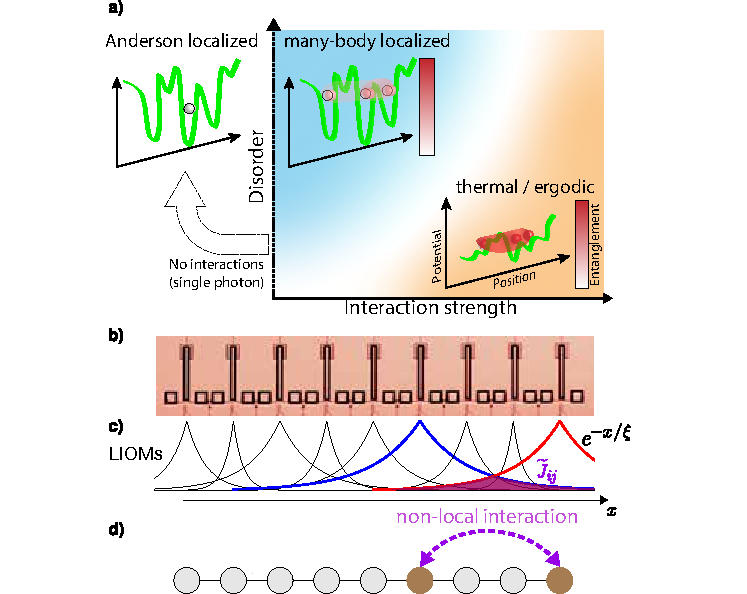
\includegraphics[width=4.5 in,keepaspectratio]{./PDF/f1_190716_1106a.pdf}
    \caption{\small
    \textbf{Many-body localization with superconducting qubits.}
    \textbf{(a)} Schematic phase diagram.
    Anderson localization for non-interacting particles occurs in 1D for arbitrarily weak disorder potentials.
    \bc{Interactions between the particles facilitate delocalization and entanglement propagation.
    When the disorder is large compared to the interaction strength, the MBL phase is realized and the particles remain localized though entanglement spreads.
    As the interactions are increased and overcome the disorder, the system transitions to a thermalized phase with fully delocalized and entangled particles.}
    \textbf{(b)} An optical micrograph of the device used in this experiment featuring $9$ superconducting qubits with tunable qubit frequencies and inter-qubit couplings.
    \textbf{(c)} Schematic of the localized orbitals in the many-body localized phase, known as local integrals of motion, that decay exponentially in space with a broad distribution of localization lengths $\xi$ and couplings $\widetilde{J}_{ij}$ between two localized integrals of motion.
    The shaded region indicates the interaction between two localized integrals of motion.
    \textbf{(d)} Illustration of effective nonlocal interactions on a chain of $9$ qubits.
    }
    \label{fig_1}
\end{figure}

In 1958 P.W. Anderson introduced the concept of localization
and showed that for a disordered and isolated system the electronic wave-functions can change their structure from being extended to exponentially localized.
Consequently, transport in the system is absent. % and the system will not be able to act as heat bath for its constituent parts to reach thermal equilibrium, in the absence of interactions. %MK: non-interacting particles can never thermalize
For non-interacting quantum particles Anderson localization is well understood;
it results from the quantum interference between multiple paths that are associated with elastic scattering from random potentials.
This localized phase has been experimentally observed for systems of non-interacting phonons, photons, and matter-waves.\autocite{Billy2008, Weaver1990, Wiersma1997, Schwartz2007} % Billy matter-waves, Weaver phonons,

However, recent work suggests that localization may persist even with the introduction of small interactions between particles,
thus establishing the concept of many-body localization (MBL) as a robust, non-ergodic phase of matter at finite temperature.\autocite{Basko2006, Gornyi2005, ImbriePRL2016}
Various experimental studies show that some characteristics of the MBL phase resemble a conventional non-interacting Anderson phase in which relaxation is absent\autocite{BlochMBL2015, demarco2015, Monroe2015, GrossScience2016, Bordia2017, Roushan2018, Lukin2019};
both Anderson localized and MBL phases do not thermalize.
Yet, theoretical studies suggest that the MBL phase has very different dynamical properties.\autocite{Huse2007, Bardarson2012, Huse2014, Serbyn2013, Antonello2017, Serbyn2014, Yasaman2015,  Gopalakrishnan2015, Serbyn2015, ImbriePRL2016}
In particular, resulting from the interaction between particles it is anticipated that local dephasing arises during the coherent closed-system dynamics, distinct from the commonly considered dephasing of a qubit coupled to a noisy environment.
It has been predicted that this dephasing leads to the slow growth of entanglement entropy in the MBL phase.

\afterpage{\FloatBarrier}

\begin{figure*}[!t]
    %\includegraphics[width=550 pt, keepaspectratio]{./PDF/fig_2v2_i_190619_508p.pdf}
    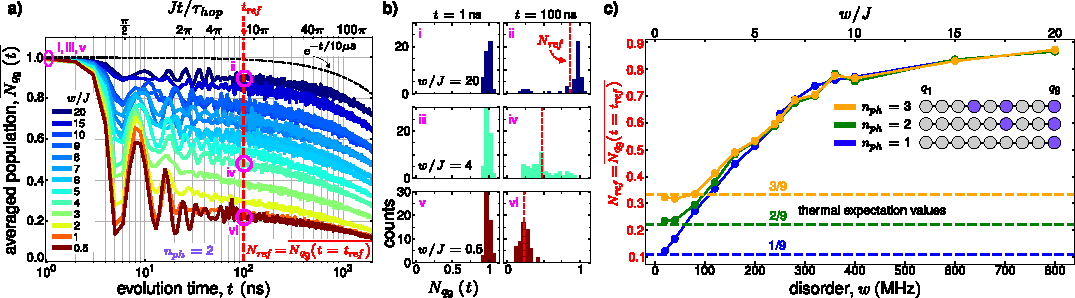
\includegraphics[width=550 pt, keepaspectratio]{./PDF/f2_190731_237p.pdf}
    \caption{\small
    \textbf{Breakdown of ergodicity.}
    \textbf{(a)} Disorder averaged on-site population \bc{vs.} time for $\bc{n_{ph}}=2$.
    In a chain of 9 qubits, two qubits were excited ('q6', 'q9').
    The on-site population of 'q9' was measured \bc{vs.} time with resolution of $\ket{0}$, $\ket{1}$, $\ket{2}$ for various magnitudes of disorder $w/J$, with $J=40 \, \text{MHz}$.  % and $U=\,$ nominally $160 \, \text{MHz}$
    Each data point is the average of 50 realizations.
    The parameter $\tau_{hop}=\hslash/J$ has been introduced to connect the laboratory time $t$ with the hopping energy.
    $N_{ref}$ is defined to be the average on-site population across instances of disorder at the reference time $t_{ref}=100\,\text{ns}$, \bc{after initial transients have been damped}.
    The dashed black line indicates expected photon loss for a single qubit measured in isolation.
    \textbf{(b)} Histograms of \bc{$\nqninet$}  at the times and disorders indicated in \textbf{(a)} by numerals i - vi. %\langle \rangle
    \textbf{(c)} $N_{ref}$ \bc{vs.} disorder for $\bc{n_{ph}}=1, 2, 3$.
    Inset shows which qubits were excited at $t=0$ ns.
    }
    \label{fig_2i}
\end{figure*}
\afterpage{\FloatBarrier}

%%%%%%%%%%%%%%%%%%%%%%%%
%%%%%%%%%%%%%%%%%%%%%%%%  Discussion of Schematic
%%%%%%%%%%%%%%%%%%%%%%%%



Using $9$  superconducting qubits, we construct a 1D bosonic lattice and study the dynamics of its micro-wave photon excitations as a function of disorder.
Each of our qubits can be thought of as a nonlinear oscillator. The Hamiltonian of the chain is described by the Bose-Hubbard model
\vspace{-8pt}
\begin{eqnarray}
    H_{BH} &=& \underbrace{\sum\limits_{n=1}^{\bc{n_Q} = 9} h_n a^{\dagger}_{n}a_{n}}_{\text{on-site detuning}} +
    \underbrace{\frac{U}{2}\sum\limits_{n=1}^{\bc{n_Q}} \,a^{\dagger}_{n}a_n(a^{\dagger}_{n}a_n-1)}_{\text{Hubbard interaction}} \nonumber \\
    &+& \underbrace{\sum_{n=1}^{\bc{n_Q}-1}J_n \left( a^{\dagger}_{n+1}a_n+a^{\dagger}_{n}a_{n+1} \right) }_{\text{NN coupling / hopping}},
\end{eqnarray}
\noindent
where $a^{\dagger}$ ($a$) denotes the bosonic creation (annihilation) operator, $h_n\in \left[ -w, w \right]$ is the random on-site detuning drawn from a uniform distribution of width $2w$,
$J$ is the hopping rate between nearest neighbour lattice sites, $U$ is the on-site Hubbard interaction, and $\bc{n_Q}$ is the number of qubits.
The qubit frequency, the nearest neighbor coupling, and nonlinearity set $h_n$, $J$, and $U$, respectively.
In our system we are able to tune each $h_n$ and $J_n$ independently at a fixed nonlinearity $U=160$ MHz.
In these experiments we set a uniform coupling across the chain $J_n = J$.

The localized regime is obtained when the frequency detunings $h_n$ are large compared to the couplings $J$.
In this regime, the eigenstates of the Hamiltonian are product states of localized orbitals, referred to as local integrals of motion (LIOMs), which are nearly qubit states but have a spatial extent that decays exponentially across the neighboring qubits.
In the localized regime, the Hamiltonian Eq (1) can be brought into a diagonal form by a set of local unitary transformations~\autocite{Serbyn2013, Huse2014}.
In order to preserve the dimension of the Hilbert space of the Bose-Hubbard model, we assume that the LIOMs are in general operators with longer spins.
In this basis there is no hopping and the Hamiltonian can be written in terms of on-site detunings and a non-local interaction.
\begin{equation}
    \tilde{H}_{\tau} = \underbrace{\sum_i \widetilde{h}_i \tau^z_i}_{\text{on-site detuning}} + \underbrace{ \sum_{i,j} \widetilde{J}_{ij}\tau^z_i\tau^z_j + \sum_{ijk} \widetilde{J}_{ijk}\tau^z_i\tau^z_j\tau^z_k + \mathellipsis.}_{\text{non-local interaction}}% = \sum_i \delta_i \left( \tau^z_{j \neq i}\tau^z_i \right).
\end{equation}
The LIOM $\tau^z_j$ commutes with $\tilde H_{\tau}$ and is hence a conserved quantity. As a consequence the system is localized.
%Thus the set $\{ \tau^z_i \}$ are referred to as local integrals of motion (LIOMs).
However, the non-local interactions $\widetilde{J}$, which follow a broad log-normal distribution,\autocite{Varma2019} spread entanglement throughout our localized system.

%%%%%%%%%%%%%%%%%%%%%%%%
%%%%%%%%%%%%%%%%%%%%%%%%  Discussion of population statics
%%%%%%%%%%%%%%%%%%%%%%%%

Evidence for the breakdown of ergodic dynamics can be obtained by measuring the mobility of excitations in our system.
In Fig. 2, we initialize the system with a number of microwave photon excitations $\bc{n_{ph}}$  by exciting $1$, $2$, or $3$ qubits.
We measure the population on one of the initially excited qubits as the 9 qubit system evolves under Hamiltonian~(1).
For each value of the disorder parameter $w$ we repeat the measurement for 50 realizations of disorder.
%A single disorder realization means that the qubit frequencies are taken to be independent random variables on the interval of $h$ $\in \left[ -\text{w}, \text{w} \right]$.
We use an overline throughout to indicate the average over disorder realizations with other parameters held fixed.

The disorder averaged population at the observation site \bc{$\overline{\nqninet}$} for $\bc{n_{ph}}=2$ is shown in panel (a).
We choose a reference time $t_{ref}$, in which \bc{$\overline{ \nqninet }$} approaches an asymptotic value \bc{after initial transients have been damped},
before the dynamics of our system are dominated by relaxation to the environment at large time scales, (indicated by the dashed black line)
or delocalization within our closed system driven by dephasing between the qubits\autocite{supplement,Znidaric2015, Levi2016, Fischer2016, Luschen2017, vanNieuwenburg2017}.
The distribution of \bc{$\nqninet$} for selected disorder magnitudes at $t=1\,\text{ns}$ and $t=t_{ref}$ are shown in panel (b).
At $t=1\,\text{ns}$ the excitations have not propagated, and there is a tight distribution close to the initial values, regardless of the value of disorder.
At $t=t_{ref}$ the distribution is narrow for low disorder and becomes wider with tails at larger disorders.
This can be understood because at high disorder, level resonances are increasingly rare which inhibits mobility.
The tail of the distribution results from these rare cases.
At low disorder, all qubits are near resonance and excitations can propagate freely between them and the behavior of each disorder instance is typical.

%%%%%%%%%%%%%%%%%%%%%%%%
%%%%%%%%%%%%%%%%%%%%%%%%  Discussion of population dynamics
%%%%%%%%%%%%%%%%%%%%%%%%
\begin{figure}[tb]
        \centering
        %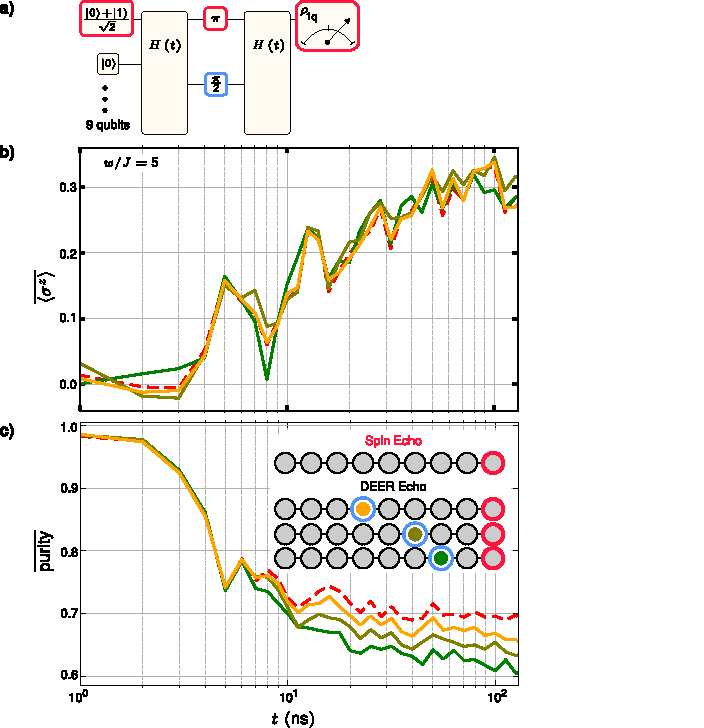
\includegraphics[width=89 mm]{./PDF/f4_190714_1032p.pdf}
        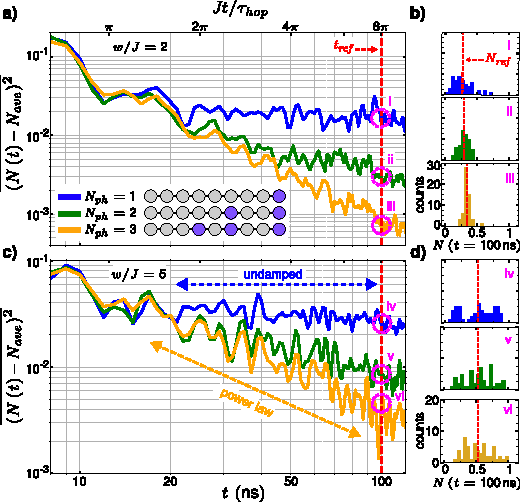
\includegraphics[width=89 mm]{./PDF/f3_190714_509p.pdf}
        %\includegraphics[width=200 pt, keepaspectratio]{./PDF/fig_2v2_ii_190408_416p.pdf}
        %\includegraphics[keepaspectratio]{./PDF/fig2_190401_146p.pdf}
        \caption{\small
        \textbf{Damping of population fluctuations.}
        \textbf{(a)}  Population fluctuations \bc{vs.} time for $w/J=2$.% and $U \,$ nominally $160 \, \text{MHz}$.
        The interacting $\bc{n_{ph}} \geq 2$ photon data (green and yellow) exhibits fluctuation damping in contrast to the noninteracting single photon case.
        \textbf{(b)}  Histograms of \bc{$N_{q_\text{9}} \left( t=t_{ref} \right)$} across instances of disorder at the points indicated in \textbf{(a)}.
        \textbf{(c)}  Population fluctuation \bc{vs.} time for $w/J=5$, in the non-ergodic regime.  The dashed lines indicating undamped behavior and power law decay are guides to the eye.
        \textbf{(d)}  Histograms of \bc{$N_{q_\text{9}} \left( t=t_{ref} \right)$} across instances of disorder at the points indicated in \textbf{(c)}.
        Data in this figure is for $J=\,40 \text{MHz}$.
        }
\end{figure}

Fig. \ref{fig_2i}(c) shows the disorder averaged population after $t_{ref}=100\, \text{ns}$ of evolution as a function of the disorder strength.
At low disorder, in the diffusive regime, we expect the dynamics to satisfy the ergodic hypothesis \bc{that each of the two photon states is equally likely to be observed.}
Here, a uniform averaging over the available phase space implies that the expected occupancy of a given qubit should be $\bc{n_{ph}}$~/~\bc{$n_{Q}$}.
For multiple photon excitations our observations are consistent with ergodic dynamics at weak disorder, however, as we increase the disorder, significant deviations from the thermal value are observed, which indicates that our system becomes many-body localized.
We note that with more photons in the system, the population converges to its thermal expectation value at higher disorders.
This is expected because the increased interactions assist with the thermalization process and drive delocalization.
In the case of a single excitation our system is effectively non-interacting and hence localized for all disorders. The apparent approach of the population to the thermal value at extremely weak disorder indicates the regime where the single-particle localization length exceeds our system size.

\begin{comment}
\textbf{
Because there is loss in our system, we do not have access to arbitrarily long time scales and we cannot conclusively demonstrate that the population has achieved an equilibrium value.
However, it is clear that at our reference time $\text{t}_\text{ref}=100$ ns at low disorders the on-site population takes its thermal expectation value and at higher disorders it fails to do so.
}
\end{comment}

The presence of interactions between distant LIOMs in Eq. (2), leads to crucial differences in the dynamics of MBL and Anderson systems.
In both the Anderson and MBL phases particle transport is absent.
However, in the MBL phase the exponential decay of interaction strength with the distance between LIOMs is responsible for exponentially slow dephasing between distant degrees of freedom.
This slow dephasing is for instance responsible for the MBL signature logarithmic-in-time growth of entanglement for initial product states \autocite{Bardarson2012, Huse2014, Serbyn2013}. Here we will elucidate the effects of dephasing on fluctuations of local observables, echo probes, and entanglement in the MBL phase using our superconducting qubit device.

As a consequence of the dephasing the temporal fluctuations of local observables are slowly damped in MBL systems and relax to highly nonthermal stationary states at long times
$\left( N_{ref} \neq \bc{n_{ph}}/\bc{N_{q}} \right)$.\autocite{Serbyn2014}
By contrast, in Anderson localized systems, local observables generally do not relax, but oscillate in time perpetually.
In Fig.\, 3 we show this fluctuation damping by inspecting the fluctuation of on-site population \bc{$\overline{ \left( \nqninet - N_{ave} \right)^2 }$} for $\bc{n_{ph}}=1,2,3$.
$N_{ave} = \left< \bc{\nqninet} \right>$ is computed for each disorder instance and the averaging is performed over a window from $t_{ref}=\text{100}\,\text{ns}$ to $\text{140}\,\text{ns}$, in order to smooth oscillations.

In (a),  after the transient behavior at short times, we observe undamped behavior for the $\bc{n_{ph}}=1$ non-interacting case and stronger damping with increasing photon number due to interactions.
The distribution of \bc{$N_{q_\text{9}} \left( t=t_{ref} \right)$} for $\bc{n_{ph}}=1,2$, and $3$ is shown in panel (b).
These histograms illustrate that promoting interactions by increasing the photon number tends to narrow the distribution around $N_{ref}$.
We note that at this disorder, $w/J=2$, Fig. 2(c) shows that for $\bc{n_{ph}}=3$,
\bc{$\overline{\nqninet}$} has achieved it's thermal expectation value,
and in Fig. 3(b) we see that the distribution is narrow around that value.
Together Figs. 2(c) and 3(b) indicate that the system is thermalizing, and that fluctuation damping due to interactions is also relevant to the thermal regime.
In Fig. 3(c) $w/J=5$ for which Fig. 2(c) suggests that the system is well in the localized phase.
Again for $\bc{n_{ph}}=1$ there are no interactions and the fluctuations are undamped, as expected for Anderson localization.
With $\bc{n_{ph}}\geq 2$ damping of the fluctuation is evident even in the localized regime, consistent with a power-law damping predicted in \cite{Serbyn2014}, as the system converges to a non-thermal stationary value.

\begin{comment}
    \textbf{
We note that if the timescale of the damping is fast relative to the timescale over which the system approaches $\text{N}_{\text{eq}}$ we can characterize the variance about $\text{N}_\text{{ref}}$ even though the population has not saturated.
    }
\end{comment}

%%%%%%%%%%%%%%%%%%%%%%%%
%%%%%%%%%%%%%%%%%%%%%%%%  Discussion of Echo
%%%%%%%%%%%%%%%%%%%%%%%%
\begin{figure}[tb]
    \centering
    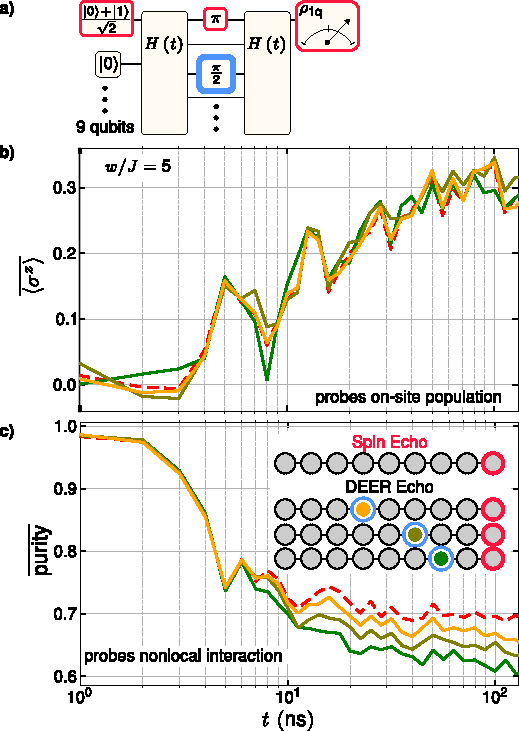
\includegraphics[width=89 mm]{./PDF/f4_190731_416p.pdf}
    \caption{\small
    %Echo sequence to probe remote entanglement
    %Interferometric probe of entanglement.
    \textbf{Interferometric signatures of remote entanglement.}
    \textbf{(a)} SE and DEER pulse sequences.
    DEER differs from SE by the addition of a remote $\pi / 2$-pulse simultaneous with the SE $\pi$-pulse between the free precession intervals.
    \textbf{(b)} $\overline{ \left< \sigma^z \right> }$ for SE (red dashed lines) and DEER (solid lines) experiments.
    \bc{$\overline{ \left< \sigma^z \right> }$ reports on-site population.  The lack of dependence on the DEER pulse indicates localization.}
    \textbf{(c)} Purity of the single qubit density matrix following the SE and DEER pulse sequences.
    \bc{The remote DEER pulse induces dephasing, decreasing the purity.
    Thus, the contrast between SE and DEER probes the non-local interaction $\widetilde{J}_{ij}$ between the SE lattice site and the DEER site.}
    Data in this figure is for $J=\,40 \text{MHz}$.
    }
    \label{fig_3}
\end{figure}
\afterpage{\FloatBarrier}

In Fig. 4 we use interferometric methods adopted from NMR to unambiguously establish nonlocal interaction effects between the LIOMs.\autocite{KnapPRL2014}
Panel (a), illustrates a conventional spin-echo (SE) sequence and its extension double electron-electron resonance echo (DEER) which we use to provide a differential measurement of phase accumulation with and without a remote perturbation.
Our protocol differs from \cite{KnapPRL2014} in that, at the end of the sequence,
rather than apply a single gate to project the bloch vector onto the quantization axis and reporting the final $\left< \sigma^z \right> = \left< 1 - 2 a^{\dagger} a \right>$, we measure the full single qubit density matrix.
This makes our technique robust against imprecision in the phase of the final microwave gate,
and at the same time allows us to verify that the non-local interaction signature we observe is not due to population transfer.

The construction of these pulse sequences can be understood from Eq. 2.
Deep in the MBL phase, the LIOMs are nearly localized on individual qubits.
The SE $\pi$-pulse between free precession intervals essentially negates the local frequency detuning, reversing the evolution and hence phase accumulation.
The role of the additional $\pi/2$-pulse in the DEER sequence is to make the SE refocusing incomplete, directly probing the strength of the nonlocal interaction.
The measurement of on-site population, depicted in panel (b), shows that the remote $\pi / 2$-pulse in the DEER sequence does not appreciably alter the population on the observation site,
assuring that the system is in the localized regime.
Therefore, comparing SE and DEER, the contrast observed in the single qubit purity, shown in panel (c), is a direct measure of nonlocal interaction between distant, localized sites in our system.
In addition, the difference between SE and DEER decreases as the distance between the SE site and remote disturbance site is increased.
This can be understood from decaying nature of the interactions between the LIOMs with distance.
The interferometric protocol is thus capable of measuring the foundational interaction effects of MBL states.



%%%%%%%%%%%%%%%%%%%%%%%%
%%%%%%%%%%%%%%%%%%%%%%%%  Discussion of Log growth
%%%%%%%%%%%%%%%%%%%%%%%%

\begin{figure}[tb!]
    \centering
        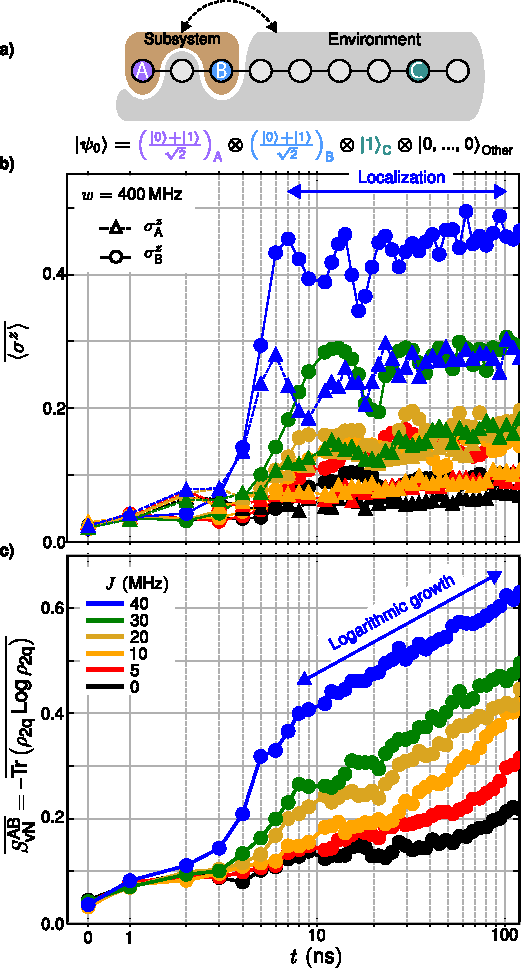
\includegraphics[width=250 pt, keepaspectratio]{./PDF/f5_190716_156p.pdf}
        \caption{\small
        \textbf{Localization and logarithmic growth of entanglement}
        \textbf{(a)} Schematic diagram showing the partitioning of our 9-qubit chain into a sub-system and environment.
        The sub-system qubits (A and B) are initialized into superposition states,
        and the system is loaded with an additional excitation (site C) to enhance many-body interactions.
        We tomographically reconstruct the  density matrix of the two qubit sub-system.
        \textbf{(b)} On-site $\overline{\left< \sigma^z \right>}$ for sub-system qubits (A and B).
        \textbf{(c)} von Neumann entanglement entropy of the two qubit sub-system for several coupling strengths. %\mkch{I see now the problem with the $2\pi$. We could solve it by labeling in Fig. 2 the time axis as $Jt/\hbar$. Then you can normally write the coupling in MHz.}
        }
        \label{fig_4}
\end{figure}

%The definitive measure of entanglement with the environment is to compute the von Neumann entropy from the density matrix.
The hallmark of the MBL phase is the logarithmic-in-time growth of entanglement in spite of localization, contrasting it with non-interacting Anderson localization where the entanglement is constant.
To study the development of entanglement entropy, we designate two qubits as a sub-system and the rest of the chain as the environment, as shown in panel Fig. 5(a).  %we embed a two qubit sub-system in a many-body localized environment and observe its evolution.
We directly measure the evolution of the reduced density matrix of the sub-system.
The sub-system qubits are initialized into superposition states, which enhances the measurement visibility by being highly phase sensitive.

%Fig. 5 (b) shows that
%$\overline{ \left< \sigma^z \right> }$ initially rises as population from the sub-system qubits hops into the neighboring environmental qubits.
%After this initial rise, $\overline{ \left< \sigma^z \right> }$ takes a stationary value, establishing the localization of our system.

Fig. 5 (b) shows that$\overline{ \left< \sigma^z \right> }$ initially rises because population from the subsystem qubits is transferred to the environment which has a smaller photon density.
After this initial rise, $\overline{ \left< \sigma^z \right> }$ takes a stationary value which decreases with increasing disorder, establishing the localization of our system.

We use the von Neumann entanglement entropy
\begin{equation}
    S_{\text{vN}}=-\text{Tr} \rho_{\text{2q}} \text{log} \rho_{\text{2q}}
\end{equation}

\noindent to quantify the entanglement between the sub-system and the environment (Fig. \ref{fig_4}(c)).
The initial increase in $\overline{ S_{\text{vN}} }$ occurring simultaneously with the increase in $\overline{ \left< \sigma^z \right> }$ is understood as the sub-system entangling with the environment by performing a partial swap.
Thereafter, while the system is demonstrably localized, we observe logarithmic-in-time growth of von Neumann entanglement entropy.

We can understand the logarithmic growth of the entanglement entropy in terms of the LIOM framework: The non-local and exponentially decaying interactions between the LIOMs give rise to dephasing between the qubits and follow a broad log-normal distribution.~\autocite{Varma2019} As a consequence, the entanglement of individual runs is strongly fluctuating on different time scales leading to an on average logarithmic growth of the entanglement even for our two qubit subsystem.

\begin{comment}
The LIOM framework provides a simple explanation for this result: The non-local and exponentially decaying interactions between the LIOMs give rise to dephasing on a hierarchy of exponentially large time scales.
Inverting that, we can estimate that the system becomes entangled logarithmically in time.
This logarithmic entanglement growth is a hallmark of many-body localized systems and signifies a true interaction effect, which supports the comparisons between the DEER echo and spin echo measurements in Fig. 4.
\end{comment}

Preparing subsystem qubits in an x-polarized state enhances the strength of the entanglement growth and hence its logarithmic behavior can be clearly observed in our system.
Note that the small rise of the entanglement entropy in the case of uncoupled qubits $\left( J=0 \right)$ at late times (black) comes from mixing in our system, which is however negligibly small up to $\sim50\,\text{ns}$, at which we already see a clear signature of the logarithmic entanglement growth.



%%%%%%%%%%%%%%%%%%%%%%%%
%%%%%%%%%%%%%%%%%%%%%%%%  Discussion of Memory
%%%%%%%%%%%%%%%%%%%%%%%%

\begin{figure}[tb!]
    \centering
        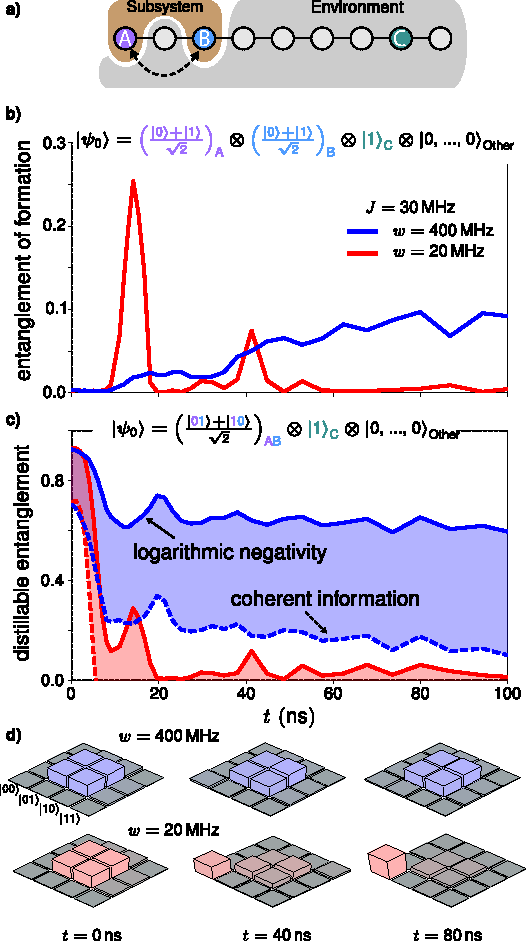
\includegraphics[width=89 mm, keepaspectratio]{./PDF/f6_190716_1129a.pdf}
        \caption{\small
        \textbf{Growth and preservation of entanglement between localized sites}
        \textbf{(a)} Schematic diagram emphasizing our focus on the entanglement between qubits A and B which are embedded in an environment.
        \textbf{(b)} \bc{To observe the development of entanglement between sites A and B} the sub-system is initialized in a product of single qubit superposition states and the entanglement of formation of the two qubit density matrix is extracted.
        \textbf{(c)} \bc{We demonstrate the capability of the MBL phase to preserve entanglement initializing the sub-system into a maximally entangled Bell pair and observing the decay of quantum correlations.}
        We extract the logarithmic negativity and coherent information from measurements of the two-qubit sub-system density matrix.
        These provide, respectively, upper and lower bounds on the distillable entanglement within the sub-system.
        \textbf{(d)} Representative density matrices from single disorder instances contained in \textbf{(c)} at high and low disorder.
        }
        \label{fig_5}
\end{figure}
\afterpage{\FloatBarrier}

We will now investigate the formation and preservation of entanglement between two qubits A and B that are embedded in a many-body localized environment as illustrated in Fig. 6(a).
%From the quantum information point of view it is interesting to know how entanglement develops between specified sub-system qubits.
%We therefore emphasize measures that describe the entanglement between parts of the sub-system in Fig. 6 as illustrated in panel (a).
The entanglement of formation quantifies the amount of entanglement directly between qubits A and B that would be required to produce the observed two-qubit mixed state density matrix.\autocite{Wootters1998}
In panel b), we initialize the sub-system into an unentangled product state of single qubit superpositions and observe the development of entanglement between our sub-system qubits.
At high disorder, associated with the localized phase, entanglement grows continuously between the spatially separated sites.
At low disorder, corresponding with the ergodic phase, we observe brief intervals of significant entanglement as the excitations delocalize across the full 9 qubit system.
However, this behavior is quickly damped as the excitations are absorbed by environmental qubits, as the full 9-qubit system thermalizes.

While the results discussed thus far show interaction effects between the LIOMs, it is also a major prospect to demonstrate the preservation of quantum information in such a system.
To this end, we prepare a distant Bell state between the first and the third qubit and study the entanglement dynamics.
While dephasing between LIOMs will ultimately destroy the entanglement, it will only due so on exponentially long times due to the localization.
Crucially, the subsystem is in a mixed state, because it is coupling to the other 7 qubits of our device.
We therefore characterize the entanglement of the 2-body mixed density matrix $\rho_{2q} \left( t \right)$ using an operational entanglement measure.
In particular, we focus on the distillable entanglement, i.e., the entanglement which can be extracted from the mixed density matrix, that is upper bounded by logarithmic negativity entropy and lower bounded by the coherent information entropy.
These bounds are shown in panel (c). For weak disorder (red), the prepared quantum information is immediately lost because the quantum dynamics entangles the subsystem with its environment and a featureless high temperature state is attained locally.
%
This behavior can also be understood in terms of the monogamy of entanglement.\autocite{Wootters2000}
Although the two qubit subsystem is initially prepared in a maximally entangled state the degree of quantum correlation between subsystem sites decreases as the subsystem exchanges information with the environment and entangles with it.
This monogamic principle also explains the damping of the peak in the low disorder data of panel (b).
%
However, for strong disorder (blue) the distillable entanglement is sizable over long times, and hence the density matrix can be used as quantum resource.
This is exemplified in panel (d) which shows the tomographic reconstruction of the two qubit density matrix for a single disorder instance as it evolves in time.
These results show that a many-body localized system can efficiently retain quantum information over long time scales.

The experimental capabilities in systems with superconducting quibts to perform a wave function initialization, Hamiltonian generation, and measurements in different bases allows us to perform a comprehensive study of interaction effects in the many-body localized phase.
In particular, by creating superposition states and performing full tomography on subsystems we are able to capture elusive phenomena of many-body localization such as the entanglement dynamics and interferometric signatures.
These techniques may allow us to study foundational aspects of clean quantum many-body systems including the growth of operators as characterised by out-of-time ordered correlators and entanglement phase transitions.

\begin{comment}
The primary challenge of creating a powerful quantum simulation platform is in the simultaneous realization of
on-demand wavefunction initialization, Hamiltonian generation, and measurement in different bases.
Understandably, the generation of many-body Hamiltonians has been a significant research focus of the quantum simulation field.
However, this work highlights the complementary importance of choice of initial state and measurement observable.
Our experimental platform, which has been engineered to provide all of these capabilities,
permits us to produce a comprehensive phenomonalogical survey of entanglement dynamics in a many-body localized system.
Specifically, our ability to directly initialize specified excitations, superpositions, and Bell pairs, evolve under many-body Hamiltonians generated on demand, and tomographically measure subsystem density matrices
lead to our ability to capture such diverse and ellusive facets of many-body localization as fluctuation damping, effective nonlocal interaction, and the direct observation of development and preservation of entanglement between separated sites in a localized system.
\end{comment}

\vspace{3mm}
\footnotesize
Acknowledgements:  The authors acknowledge valuable conversations with Jens Eisert and Andrew Daley.
M.K. and A.B. acknowledge support from the Technical University of Munich - Institute for Advanced Study, funded by the German Excellence Initiative and the European Union FP7 under grant agreement 291763, the Deutsche Forschungsgemeinschaft (DFG, German Research Foundation) under Germany's Excellence Strategy--EXC-2111--390814868, DFG grant No. KN1254/1-1, and DFG TRR80 (Project F8).

